\documentclass[a4paper,12pt]{report}
\usepackage{graphicx}
\usepackage{times}
\usepackage[a4paper,total={6in,8in}]{geometry}
\usepackage{multirow}
\usepackage{caption}
\usepackage{blindtext}

\begin{document}

{\centering \bf \large
	WORKLORD\par
}
\begin{center}
	{\small PROJECT REPORT} \vspace*{10pt}
	\\ Submitted by\\
	\vspace*{15pt}
	{\bf MOHAMMED ALTHAF T\\
\vspace*{8pt}	LKMC18MCA026\\

\vspace*{8pt}ANJUSHA BJ\\
\vspace*{8pt}KMC18MCA002\\
	\vspace*{20pt}
	to}\\
	\vspace*{13pt}
	the APJ Abdul Kalam Technological University in partial fulfillment of
	the requirements for the award of the Degree\\
	\vspace*{10pt} of\\
	\vspace*{10pt} \textit{ Master of Computer Applications
	} 
\vspace*{10pt}
\begin{figure}[bph]
	\centering
	
\includegraphics[width=0.3023\linewidth]{kmct}
	\label{fig:ksblogo}
\end{figure}

	\bf{Department of Management Studies  Computer Applications
	\vspace*{15pt}
	\\KMCT College of Engineering
	\vspace*{10pt}
	\\Kallanthode, NITC P.O, Kozhikode-673601}

\end{center}
	\begin{center}
		\vspace*{15pt}AUGUST 2020
	\end{center}


\pagebreak

\addcontentsline{toc}{section}{ABSTRACT}
\section*{\centering \bf \large ABSTRACT}
\vspace*{20pt}
\par
\hspace*{12pt}Technology has changed the way job seekers search for jobs and employers
find qualified employees. While employers still advertise job openings through
traditional advertising mediums, today employers and job seekers turn to online
job portals to find employment matches. Job seekers can advertise their skills and
search for available positions and employers can announce employment openings
through job portals.\\

The proposed system ”WORK LORD” is a web based application to give the
job seekers a platform for finding right and satisfactory job according to their qualification and skills. It also connect the job seekers with the major companies. This application is mainly focused on the applicants, who are seeking jobs in CS (Computer
Science) field. Job seekers can register themselves with resume at the website where as the
employers register in the website and put job vacancies at their
company. Employers can also browse through the posted resumes and user performance. The system provides jobs catalogue and information to members. The Admin and employers can
keep the catalogue updated all the time so that the job seekers get the updated information all the time.\\

There are many job portals that claims to provide you the best job, but none
of them address the issues faced by the job seekers. They face issues because of work experience, because Companies give more priority for experienced job seekers. And they are not calculating the skill level of the job seekers. In this project we provide the Job Seeker to express their skills by completing the tests provided by admin which helps employer to understand their skills in their fields easily. Also they will
be getting tasks to complete for measuring their performance. Most
scored/skilled persons will be highlighted top and gets faster job opportunities such as preferred employer, preferred technology should be there. Calculating skills will be a great option for freshers to seek jobs. The issues faced by freshers can solved by implementing these features in the web application. The priority based oppertunities can be avoided by this. In our project we will be focusing on changing
such attitude towards freshers.\\


\pagebreak

\chapter{INTRODUCTION}

\hspace*{12pt}The quality of people hired for a specific job is usually the key issue when measuring the effectiveness of the employment. However, in certain circumstances the speed of hiring is also an issue and also contribute to quality hiring. The rationale of a hiring process is to stretch out to potential employees and bring out the specific kind of required skills and experiences in the field organization. Online job portal system is fundamental in removal of paper works and introduction of workflow systems that connect job seekers and employers. At a very low cost, the internet offers employers and job searchers access to detailed and up-to-date information about job vacancies in different locations around the world. \\

WORKLORD project is aimed at developing a job portal friendly for non-experienced and experienced job seekers. The system project is an online web application which can be accessed from anywhere only with a proper login verification. Job seekers should be able to login and upload their resume and update their contact details. There are many job portals that claims to provide you the best job, but none of them address the real issues faced by the non-experienced job seekers. Companies give higher priority for experienced job seekers. They failes calculate the skill level of the job seekers. \\

 In this project we insist the Job Seeker to complete specific tests provided by the admin which helps employer to understand job seeker's skills and performance in their fields. Also they will be getting tasks to express their performance and efficiency. Most scored/skilled persons will be getting more priorities, Options such as top scored candidate, preferred employer, preferred technology should be there. Calculating skills will be a great option for freshers to seek jobs. The issues faced by the new job seekers to find a perfect job with their skills is difficult. In our project we will try to change such attitude from companies towards freshers. This system gives the company to search for the best candidate available on the fields.\\

\pagebreak

\chapter{SYSTEM ANALYSIS}
\section{Existing system}

\hspace*{12pt}The traditional hiring of employees starts with the processing of application forms, describe the job for each position, verify application forms and lastly evaluate the best person for the job. The whole process from advertisement to hiring a quality applicant takes a lot of time, effort and also has more weakness. The advertisement itself is costly especially when done through print media. therefore, the publication of the job adverts will only last for a very short time and in that case few people will have seen the job vacancy. Thus, the traditional recruitment process is not be the best in today's competitive job market.\\

The question here is how this could be made efficient and possible. This question or problem solved by an online job portal system which is set to transform the way in which companies and other employers recruit their employees. The Job seeker Functions concentrates on the consistent information that is practically, part of the organizational activities and which needs proper authentication for the data collection. The users can perform some tasks without registering or without entering into the application. He can search for the jobs in the site. He can view the information which is available for the job seekers. Also view the walk-in details. The job seeker can perform some tasks only after entering into the application. In any situation the job seeker needs to change his password then he can change on his own. He can view the details of his own profile and he can modify his details in his profile. The employer can view his own profile and they can also post new job vacancies and they can view the candidates resumes applied for jobs. The admin functions concentrates on maintain the functionality of site. Proper management of complete job seeker section and employer section is his responsibility.\\

\section{Proposed system}
\hspace*{12pt}
The proposed system ”WORKLORD” is a web based application is to give the job seekers a platform for finding right and satisfactory job according to their qualification and skills. It also connect the job seekers with the major companies. Job Portal is a platform that joins recruiters and the job seekers to complete their goals and requirements. Recruiters look for a right candidate who has the right qualification to handle the responsibilities efficiently. On the other  hand, job seekers want a job where they can apply their skills and knowledge to grow their professional career. Most of the jobseekers who're actively seeking new employment opportunities are believed to be registered on multiple job portals. Finding a job opportunity per your choice and qualification through a job portal is relatively easier. There are many job portals that claims to provide you the best job, but none of them address the issues faced by the new job seekers. Most of portals give higher priority for experienced job seekers.\\

Job portals requires features like profile management, view notifications and other filtering options to match with the company with their skills. The users can perform some tasks without registering like he can search for the job vacancies,walk-in details which available in the notifications section. The job seeker can perform some tasks only after registration. After registering he can attend for tests and complete tasks. He can also view and modify his profile and also he can change his password. The employer can view their profile and they can post new job vacancies. They can also view the candidates resumes applied for jobs. The admin functions concentrates on maintaining the functionality of site. Proper management of complete job seeker section and employer section is his responsibility. He also provides tasks and updates test datas. Users analytics shows you a compiled listing of all users and the time they have spent using their Skills. Users analytics is one of the more important analytics sets when they are trying to calculate skills relating to an individual. We can check into a particular individual's peformance and see how they are performing. Many companies prefer employees with good experiences and reputation in their previous job rather than freshers. This causes issues with finding jobs for freshers with right skills. In this project we will be trying to change such attitude towards freshers. This system facilitate the company to search for the best candidate available and employ them as employers to improve efficiency on the employment sector.\\

\pagebreak

\section{Module Description}
\subsection{User}

\subitem
\\ - Search for Job Posts
\\ - Apply Online for Job Posts
\\ - Attend Exams in the website
\\ - Complete Tasks
\\ - Update Profile and Resume
\\ - Send Reply to Applied Job's Company
\\ - View Application's Status
\\ - View Scores in Exams and Task

\subsection{Company}

\subitem
\\ - Add Job Posts
\\ - Review Applications
\\ - Download Applicant's Resume
\\ - Contact Applicant
\\ - View Messages from User
\\ - View Exams and Task Scores

\subsection{Admin}

\subitem
\\ - Manage Active Jobs
\\ - Manage Users
\\ - Manage Companies
\\ - Add Exams and Update Questions
\\ - Add Tasks
\\ - Review Task
\\ - View Task/Exam Scores

\pagebreak


\section{Feasibility Study}

\subsection{Operational Feasibility}

\hspace*{12pt} This Project is beneficial to people who wants to meet the qualifications of theirs and 
company's requirements. There's not much difficulty in, implementing the proposed system, It is so more effective, user friendly and functionally reliable to everyone. WORKLORD job portal is beneficial for every new job seekers, They can access this web portal from any where. This
website can be accessed from any devices like laptop or smartphone with internet connection. Any
of the user with good internet connection can register the website and complete tests and wait for right company to pick them up, users can make use of this portal by completing tasks which improves their skills.

\subsection{Technical Feasibility}

\hspace*{12pt}Technical Feasibility study deals with the hardware as well as software requirements. We have to determine whether the project done with the current technology has been examined in the feasibility study. The proposed system requires software like gedit and web server solution application called Xampp both are available for free. The website can also be easily upgraded to the higher level with less effort and maintenance. This website can be easily accessed with user's smartphone from anywhere
with internet connection and portal is very much user friendly. Hence the Proposed system is technically feasible.

\subsection{Economic Feasibility}

\hspace*{12pt}Economic feasibility determines whether the proposed system is capable of generating
profit for an organization. It involves cost incurred on the development team, estimated
cost of hardware and cost of performing feasibility study and so on, this website was developed with
the available resources. Since cost of input for the system is almost zero. The output of the website is
always a profit for the user and we see this as a service. This website doesn’t cost any charge from the job seeker who is accessing it. Since the
website can be accessed from any device with internet connection there is no need for a specific
hardware. Hence it is economically feasible.

\pagebreak

\section{System Environment}
\hspace*{12pt}
\subitem - Back-end : PHP,MYSQL(Database)\\
\subitem - Front-end : Javascript,Bootstrap,Html,CSS\\

\subsection{Minimum Requirements (User)}
\hspace*{12pt}
\subitem - Computer/Laptop/Mobile \\
\subitem - Any OS with Updated Browser \\
\subitem  - Stable Internet Access \\

\subsection{Minimum Requirements (Developer)}
\hspace*{12pt}
\subitem - Processor : Intel Pentium/Celeron or newer \\
\subitem - Memory : 2 GB RAM \\
\subitem - Storage : 20 GB HDD/SSD (Recommended) \\
\subitem - Operating System : Linux\\
\subitem - Text Editor : Gedit\\
\subitem - Web server solution : Xampp\\
\subitem - Browser : Chrome \\
\subitem - Other Utils : Git \\
\subitem - Stable Internet Access\\

\pagebreak

\section{Actor and Their Roles}
\subsection{User}

\subitem
\\ - Register
\\ - Login
\\ - Attend Tests
\\ - Complete Task
\\ - Edit User details
\\ - Apply for Jobs
\\ - Reply Messages from Company
\\ - View Scores

\subsection{Company}

\subitem
\\ - Register
\\ - Login
\\ - Edit Company details
\\ - View qualified users
\\ - Add Job Posts
\\ - Review Job Applications
\\ - Download Resumes
\\ - Send Messages to Applicants

\subsection{Admin}

\subitem
\\ - Login
\\ - View/Edit Users
\\ - Approve Companies
\\ - View/Edit Jobs
\\ - Add Exams and Update Questions
\\ - Add New Tasks
\\ - Review Tasks

\pagebreak



\chapter{METHODOLOGY}

\section{Introduction}
\hspace*{12pt}This project follows Agile methodology. Agile software development comprises various approaches to software development under which requirements and solutions evolve through the collaborative effort of self organizing and cross-sectional teams and their customers/end users. It advocates
adaptive planning, evolutionary development, early delivery and continuous improvement and it encourage rapid and flexible response to change.
\newpage
\section{UML Diagrams}

\subsection{Activity Diagram}
\vspace*{12pt}
\subitem {\centering \bf - USER}

\begin{figure}[bph]
	\centering
	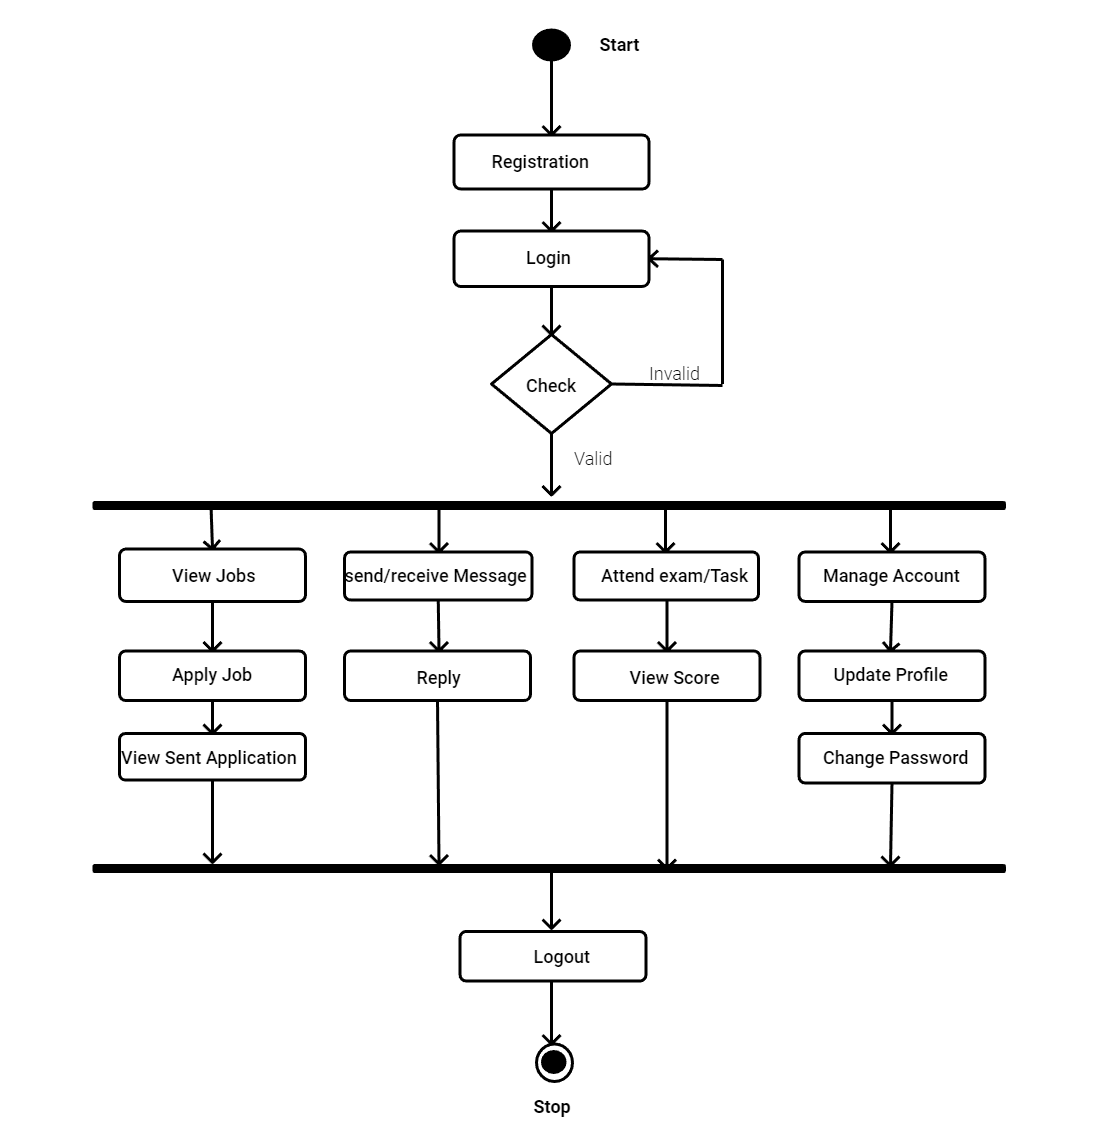
\includegraphics[width=.8\linewidth]{img/useractivity}
	\label{fig:useractivity}
    \caption{User's Activity Diagram}
\end{figure}

\pagebreak
\subitem {\centering \bf - COMPANY}
\vspace*{12pt}
\begin{figure}[bph]
	\centering
	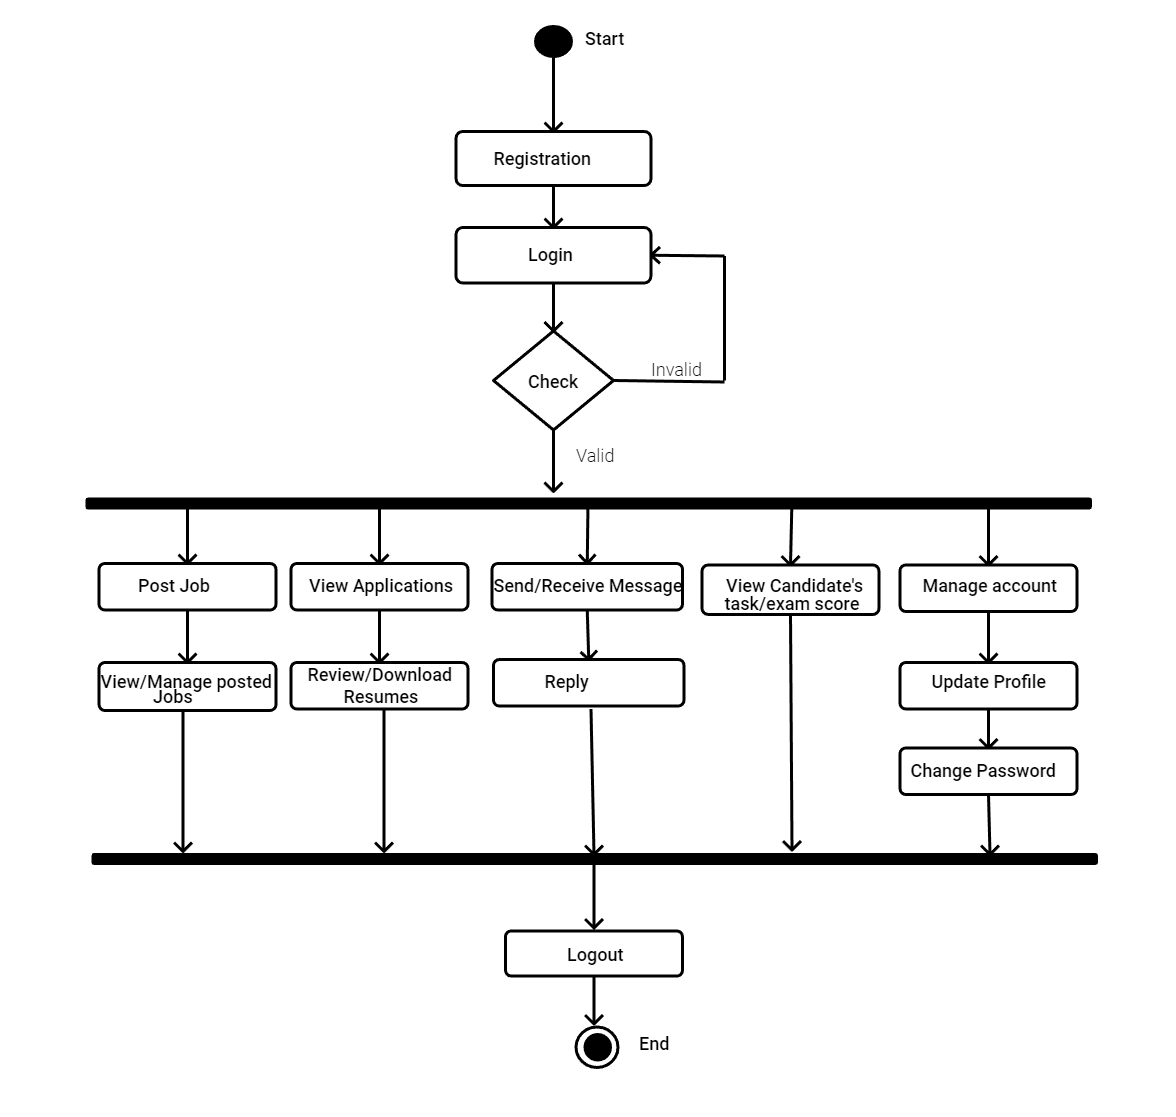
\includegraphics[width=.8\linewidth]{img/cmpnyactivity}
	\label{fig:companyactivity}
	\caption{Company's Activity Diagram}
\end{figure}

\pagebreak

\subitem {\centering \bf - ADMIN}
\vspace*{12pt}
\begin{figure}[bph]
	\centering
	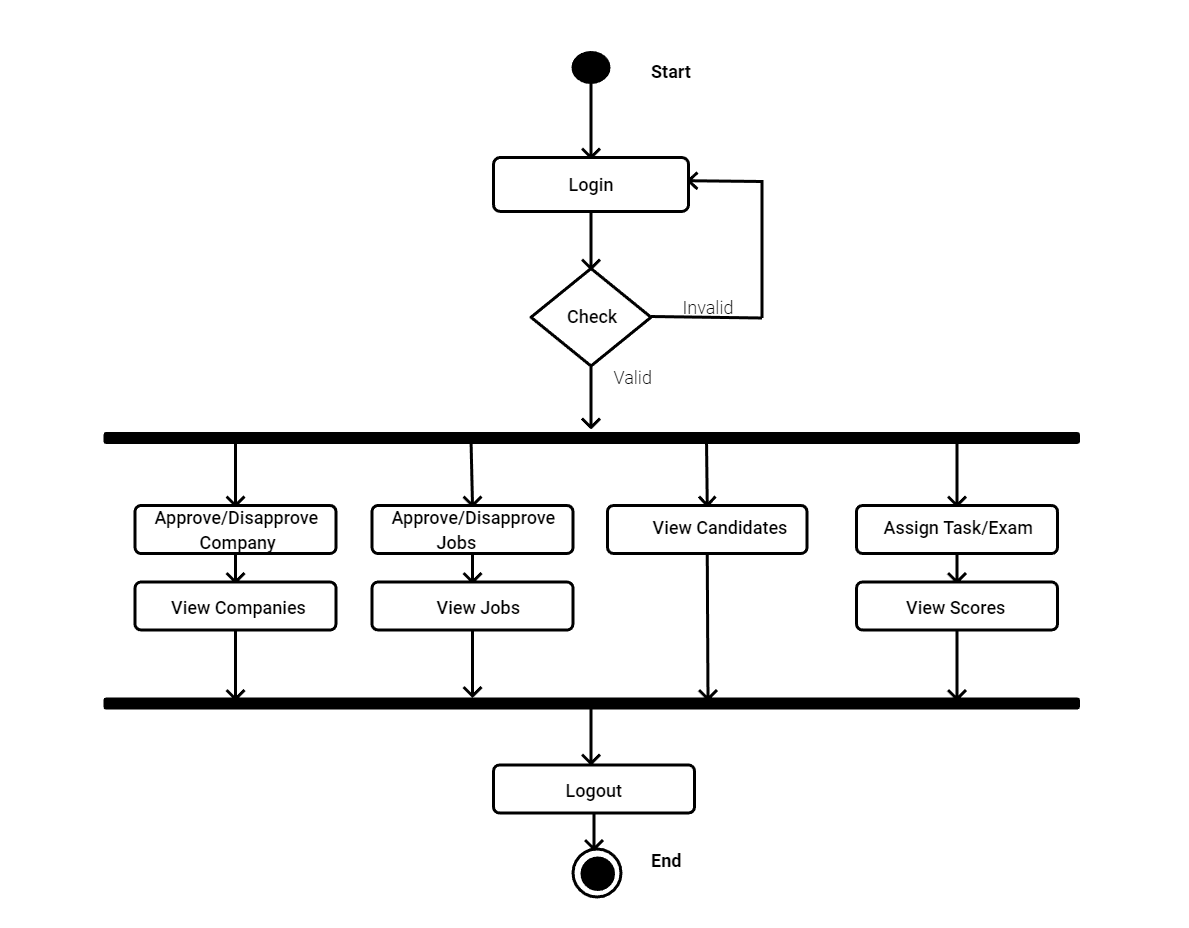
\includegraphics[width=1.1\linewidth]{img/adminactivity}
	\label{fig:adminractivity}
	\caption{Admin's Activity Diagram}
\end{figure}
\pagebreak
\subsection{UseCase Diagrams}

\vspace*{12pt}
\begin{figure}[bph]
	\centering
	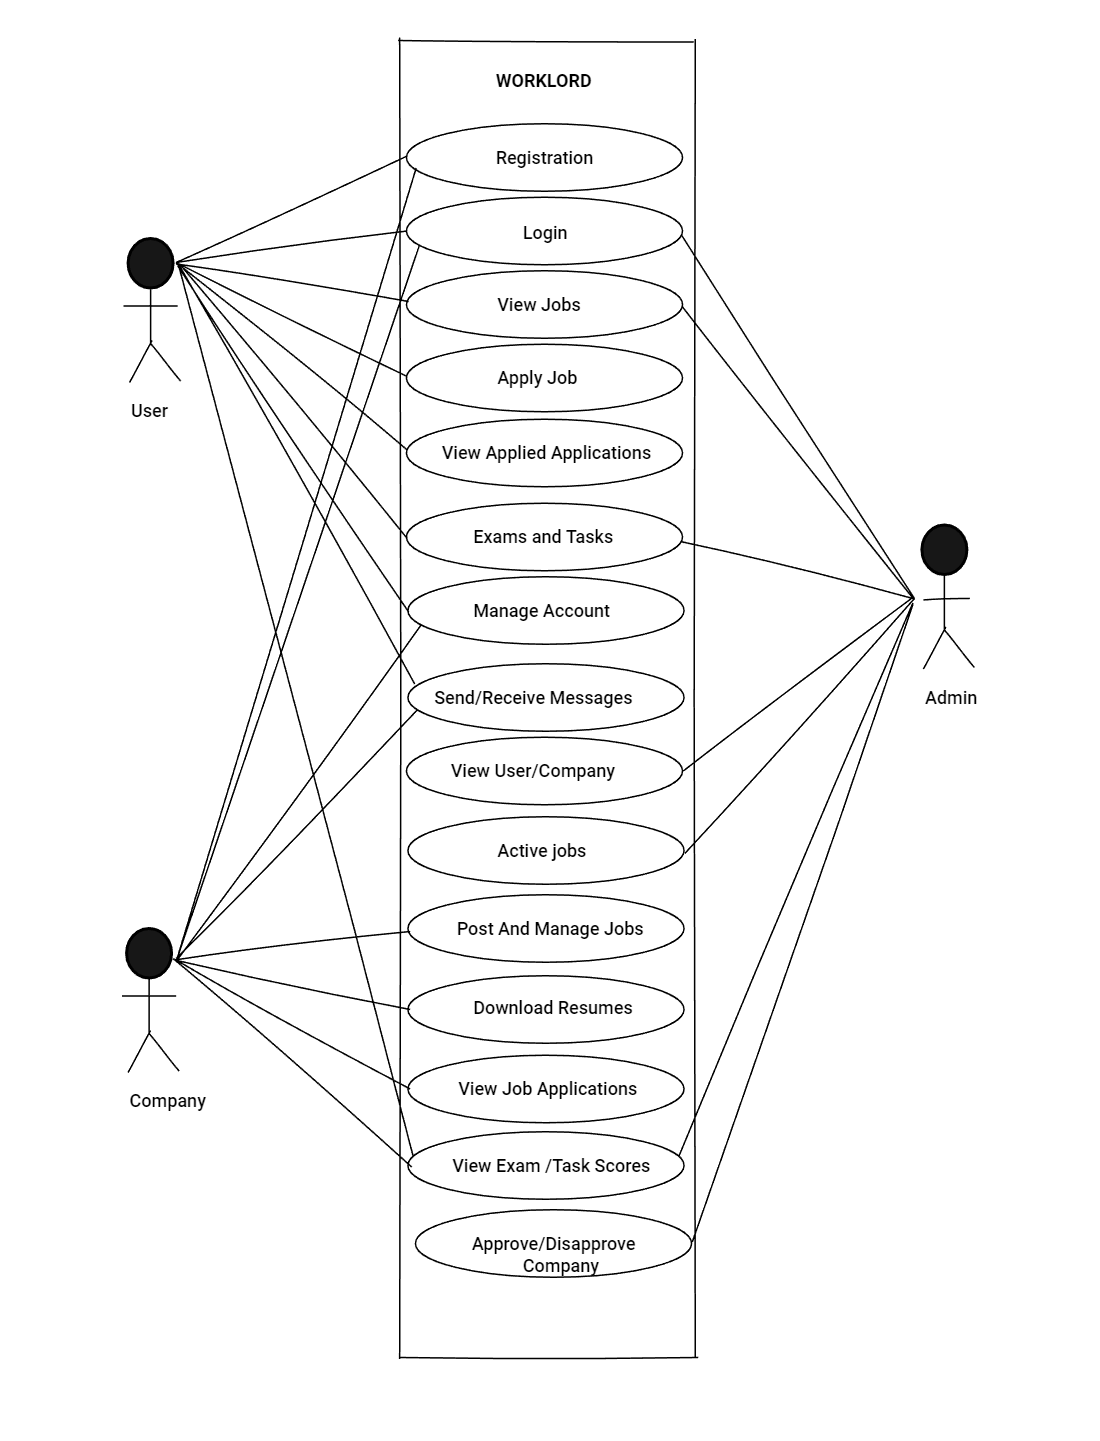
\includegraphics[width=.7\linewidth]{img/use_case_diagram}
	\label{fig:usecasediagram}
	\caption{UseCase Diagram}
\end{figure}
\pagebreak
\section{User Story}
\vspace*{12pt}

\begin{center}
	\begin{tabular}{ | p {1.5 cm} | p {4 cm} | p {3.5 cm} |  p {4.5 cm} | }
		
		\hline 
		User story ID & As a $<$Type of Users$>$ &I want to $<$Perform some task$>$ & So that I can $<$Achieve some goal $>$ \\
		\hline
		1 & Admin/User/Company & Home Page & Go to other activities\\ \hline
		2 & Admin/User/Company & Login & Access the system\\ \hline
		3 & User/Company & Registration & Access the system\\ \hline
		4 & Admin & Approve/Disapprove company & Manage companies\\ \hline
		5 & Admin & View companies & View companies\\ \hline 
		6 & Company & Post jobs & Add Job vaccancies\\ \hline
		7 & Admin & Delete Jobs & Manage jobs\\ \hline
		8 & Admin/User & View jobs & View jobs\\ \hline
		9 & Company & View posted jobs & Manage posted jobs\\ \hline
		10 & Admin & View candidates & View candidates\\ \hline
		11 & User & Apply job & Apply for job\\ \hline
		12 & User & View applications & View applied jobs\\ \hline
		13 & Company & View applications & View job applications\\ \hline
		14 & Company & Download resumes & Download applied candidates resumes\\ \hline
		15 & Admin & Create exams & Create exams\\ \hline
		16 & Admin & Assign tasks & Assign tasks\\ \hline
		17 & User & Attend exam & Attend exam\\ \hline
		18 & User & Attend task & Attend task\\ \hline
		19 & Admin/User/Company & View exam or task scores & Understand knowledge or skills of candidates\\ \hline
		20 & User/Company & Send and Receive Messages & Send/Receive Messages\\ \hline
		21 & User/Company &  Manage account & Update Profile\\ \hline
		22 & User/Company &  Manage account & Change Password\\ \hline

	\end{tabular}
	\captionof{figure}{ User Story}
\end{center}
\pagebreak
\section{ Product Backlog}

\begin{center}
	\begin{tabular}{ | p {1.3 cm} | p {2.3 cm} | p {1 cm} |  p {1.4 cm} |  p {2.5 cm} |  p {1.8 cm} |  p {2.8 cm} | }
	
	\hline
	\centering	\bf USER STORY ID &
	\bf PRIORITY
	(LOW,HIGH,
	MEDIUM)   &
	\bf SIZE &
	\bf SPRINT & 
	\bf STATUS (PLANNED,
	PROGRESSED,
	COMPLETED) &
	\bf RELEASE DATE & 
	\bf RELEASE GOAL \\
	\hline
	
	1& HIGH & 8 & \multirow{5}{*}{1}&Planned   & 15-09-2020 &Login to the system \\ \cline{1-3} \cline{5-7} 
	2& HIGH & 7 &                   &Planned   & 17-09-2020 &Access the system\\ \cline{1-3} \cline{5-7} 
	3& HIGH & 8 &                   &Planned   & 20-09-2020 &Access the account\\ \cline{1-3} \cline{5-7} 
	4& HIGH  & 8 &                   &Planned   & 24-09-2020 &Manage companies\\ \cline{1-3} \cline{5-7}
	5& MEDIUM & 5 &                   &Planned   & 27-09-2020 &View companies\\ \cline{1-3} \cline{5-7} \hline
	6& HIGH & 7 & \multirow{5}{*}{2}&Planned   & 30-09-2020 &Add job vaccanices\\ \cline{1-3} \cline{5-7} 
	7& HIGH & 6 &                   &Planned   & 03-10-2020 &Manage jobs  \\ \cline{1-3} \cline{5-7} 
	8& MEDIUM & 6 &                   &Planned   & 06-10-2020 &View jobs\\ \cline{1-3} \cline{5-7}
	9& HIGH & 10 &                   &Planned   & 09-10-2020 &Manage posted jobs\\ \cline{1-3} \cline{5-7} 
	10& MEDIUM & 6 &                   &Planned   & 11-10-2020 &View Candidates\\ \cline{1-3} \cline{5-7} \hline
	11& HIGH & 9 & \multirow{5}{*}{3}&Planned   & 15-10-2020 &Apply for job\\ \cline{1-3} \cline{5-7} 
	12& MEDIUM & 6 &                   &Planned   & 16-10-2020 &View applied jobs\\ \cline{1-3} \cline{5-7} 
	13& HIGH & 6 &                   &Planned   &17-10-2020 &View job applications\\ \cline{1-3} \cline{5-7} 
	14& MEDIUM & 6 &                   &Planned   & 19-10-2020 &Download applied candidates resumes  \\ \cline{1-3} \cline{5-7}
	15& HIGH & 10 &                   &Planned   & 23-10-2020 &Create exams\\ \cline{1-3} \cline{5-7}  \hline             
\end{tabular}
\end{center}
\pagebreak

\begin{center}
	\begin{tabular}{ | p {1.3 cm} | p {2.3 cm} | p {1 cm} |  p {1.4 cm} |  p {2.5 cm} |  p {1.8 cm} |  p {2.8 cm} | }
		
		\hline
		\centering	\bf USER STORY ID &
		\bf PRIORITY
		(LOW,HIGH,
		MEDIUM)   &
		\bf SIZE &
		\bf SPRINT & 
		\bf STATUS (PLANNED,
		PROGRESSED,
		COMPLETED) &
		\bf RELEASE DATE & 
		\bf RELEASE GOAL \\
		\hline
		16& MEDIUM & 7 &3 &Planned   & 26-10-2020 &Assign task\\ \cline{1-3} \cline{5-7}\hline
		17& HIGH & 8 &   \multirow{6}{*}{4}  &Planned   & 31-10-2020 &Attend exam\\ \cline{1-3} \cline{5-7} 
		18& HIGH & 8 &                   &Planned   & 01-11-2020 &Attend task\\ \cline{1-3} \cline{5-7} 
		19& MEDIUM & 7 &                   &Planned   & 02-11-2020 &Understand knowledge or skills of candidates\\ \cline{1-3} \cline{5-7}
		20& MEDIUM & 6 &                   &Planned   & 05-11-2020 &Send/Receive Messages\\ \cline{1-3} \cline{5-7}
		21& MEDIUM & 7 &                   &Planned   & 07-11-2020 &Update profile \\ \cline{1-3} \cline{5-7}
		22& MEDIUM & 7 &                   &Planned   & 08-11-2020 & Change password\\ \cline{1-3} \cline{5-7} \hline   
	\end{tabular}
\captionof{figure}{ Product Backlog}
\end{center}
\pagebreak
\section{Project Plan}
\vspace*{12pt}
\begin{center}
	\begin{tabular}{ | p {1.5 cm} | p {2.5 cm} | p {2 cm} |  p {2 cm} |  p {1 cm} |  p {2.2 cm} |}		
		\hline
		\centering	\bf USER STORY ID &
		\bf TASK   
		NAME     &
		\bf START
		DATE &
		\bf END
		DATE & 
		\bf DAYS &
		\bf STATUS ( TO 
		BE FILLED BY 
		SCRUM MASTER ) \\
		\hline
		
		1&\multirow{5}{*}{SPRINT 1}& 14-09-2020  & 15-09-2020  & 2 &  \\ \cline{1-1} \cline{3-6}
		2&						   & 16-09-2020  & 17-09-2020  & 2 &  \\ \cline{1-1} \cline{3-6}
		3&                         & 18-09-2020  & 20-09-2020  & 3 &  \\ \cline{1-1} \cline{3-6}
		4&                         & 21-09-2020 & 24-09-2020  & 4  &  \\ \cline{1-1} \cline{3-6}
		5&                         & 25-09-2020  & 27-09-2020  & 3 &  \\ \cline{1-1} \cline{3-6}\hline
		6&\multirow{5}{*}{SPRINT 2}& 29-09-2020  &  30-09-2020 & 2  &  \\ \cline{1-1} \cline{3-6}
		7&						   & 01-10-2020 & 03-10-2020  & 3 &  \\ \cline{1-1} \cline{3-6}
		8&						   & 04-10-2020  & 06-10-2020 & 3 &  \\ \cline{1-1} \cline{3-6} 
		9&						   & 07-10-2020  & 09-10-2020  & 3 &  \\ \cline{1-1} \cline{3-6}
		10&						   & 10-10-2020  & 11-10-2020  & 2 &  \\ \cline{1-1} \cline{3-6}\hline
		11&\multirow{5}{*}{SPRINT 3}&  13-10-2020 & 15-10-2020  & 3 &  \\ \cline{1-1} \cline{3-6}
		12&						   & 16-10-2020  &  16-10-2020 & 1 &  \\ \cline{1-1} \cline{3-6}
		13&						   &  17-10-2020 & 17-10-2020  & 1 &  \\ \cline{1-1} \cline{3-6} 
		14&						   &  18-10-2020 & 19-10-2020  & 2 &  \\ \cline{1-1} \cline{3-6}
		15&						   &  20-10-2020 &  23-10-2020 & 4 &  \\ \cline{1-1} \cline{3-6}
		16&						   &  24-10-2020 &  26-10-2020 & 3 &  \\ \cline{1-1} \cline{3-6}\hline
		17&\multirow{5}{*}{SPRINT 4}& 28-10-2020  &  31-10-2020 & 4 &  \\ \cline{1-1} \cline{3-6}
		18&						   &  01-11-2020 & 01-11-2020  & 1 &  \\ \cline{1-1} \cline{3-6} 
		19&						   & 02-11-2020  & 02-11-2020  & 1 &  \\ \cline{1-1} \cline{3-6}
		20&						   & 03-11-2020  & 04-11-2020  & 2 &  \\ \cline{1-1} \cline{3-6}
		21&						   &  05-11-2020 & 06-11-2020  & 2 &  \\ \cline{1-1} \cline{3-6}
		22&						   & 07-07-2020  & 08-07-2020  & 2 &  \\ \cline{1-1} \cline{3-6}\hline
		
		
	\end{tabular}
\captionof{figure}{ Project Plan}
\end{center}
\pagebreak
\section{Sprint Backlog Planned}
\subsection {Sprint 1}
\begin{figure}[bph]
	\centering
	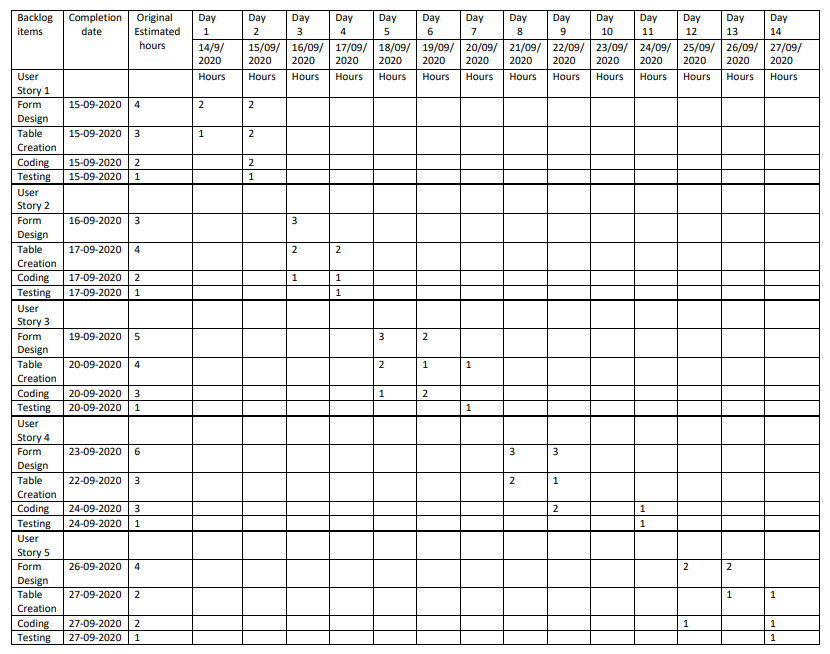
\includegraphics[width=1.1\linewidth]{img/sprint1}
	\caption{Login}
\end{figure}
\pagebreak

\section{Database Design}
\subsection{Admin Table}
This Table stores login details of Admins

\begin{center}
	\begin{tabular} { | p {1 cm} | p {3 cm} | p {3 cm} |  p {3 cm} |  p {4 cm} | }
		
		\hline
		\centering	\bf No. &
		\bf FIELD NAME &
		\bf TYPE &
		\bf CONSTRAINTS & 
		\bf DESCRIPTION \\
		\hline
		
		
		\centering	1 &adminid & INT(11) & PRIMARY KEY & Admin's ID\\ \hline
		\centering	2 &username & VARCHAR(50) & UNIQUE & Admin's Username\\ \hline
		\centering	3 &password & VARCHAR(50) & NOTNULL & Admin's Password\\ \hline
		\centering	4 &email & VARCHAR(20) & UNIQUE & Admin's Email\\ \hline
	\end{tabular}
	\vspace*{12pt}
\captionof{table}{ Admin Table}
\end{center}

\pagebreak
\section{User Interface Design}
\subsection {Homepage}
Homepage of Worklord Website
\begin{figure}[bph]
	\centering
	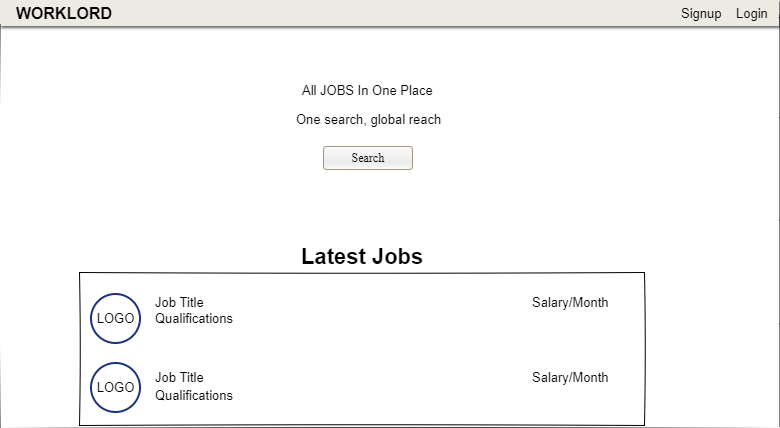
\includegraphics[width=.6\linewidth]{img/homepage}
	\caption{Homepage}
\end{figure}


\pagebreak

\end{document}
